% This must be in the first 5 lines to tell arXiv to use pdfLaTeX, which is strongly recommended.
\pdfoutput=1
% In particular, the hyperref package requires pdfLaTeX in order to break URLs across lines.

\documentclass[11pt]{article}

% Change "review" to "final" to generate the final (sometimes called camera-ready) version.
% Change to "preprint" to generate a non-anonymous version with page numbers.
\usepackage[review]{acl}
% \usepackage[final]{acl}

% Standard package includes
\usepackage{times}
\usepackage{latexsym}

% For proper rendering and hyphenation of words containing Latin characters (including in bib files)
\usepackage[T1]{fontenc}
% For Vietnamese characters
% \usepackage[T5]{fontenc}
% See https://www.latex-project.org/help/documentation/encguide.pdf for other character sets

% This assumes your files are encoded as UTF8
\usepackage[utf8]{inputenc}

% This is not strictly necessary, and may be commented out,
% but it will improve the layout of the manuscript,
% and will typically save some space.
\usepackage{microtype}

% This is also not strictly necessary, and may be commented out.
% However, it will improve the aesthetics of text in
% the typewriter font.
\usepackage{inconsolata}

% If the title and author information does not fit in the area allocated, uncomment the following
%
%\setlength\titlebox{<dim>}
%
% and set <dim> to something 5cm or larger.

\usepackage{calc}
\usepackage{amsthm}
\usepackage{amsmath}
\usepackage{caption}
\usepackage{multirow}
\usepackage{amsfonts}
\usepackage{xspace}
% \usepackage{hyperref}
\usepackage[font=footnotesize]{subcaption}
\usepackage{booktabs}
\usepackage{pdfpages}
\usepackage{xcolor}
\usepackage{tabularx}
\usepackage{bbm}
\usepackage{graphicx}
\usepackage{algorithm}
\usepackage{algorithmic}
\usepackage{enumitem}
\usepackage{pifont}

% For theorems and such
\usepackage{amsmath}
\usepackage{amssymb}
\usepackage{mathtools}
\usepackage{amsthm}
\usepackage{xspace}
\usepackage{algorithm}
\usepackage{algorithmic}
\usepackage{wrapfig}
\usepackage{enumitem}

\newcommand{\promptplaceholder}[1]{\texttt{\{#1\}}}
\usepackage[export]{adjustbox}
\newcommand{\MyEmoji}[1]{\includegraphics[width=1em,valign=t]{#1}}
% \def\red#1{{\color{red}#1}}
% \newcommand*{\red}{\textcolor{red}}
\newcommand{\red}[1]{\textcolor{red}{#1}}
\newcommand{\blue}[1]{\textcolor{blue}{#1}}
\newcommand{\ours}{\textsc{SAGE-OPD}\xspace}

\newcommand{\zz}[1]{{\color{magenta}[ZZ: {#1}]}}
\newcommand{\yz}[1]{{\color{red}[YZ: {#1}]}}

\newcommand{\defref}[1]{Definition~\ref{#1}}
\newcommand{\tabref}[1]{Table~\ref{#1}}
\newcommand{\figref}[1]{Fig.~\ref{#1}}
\newcommand{\eqnref}[1]{\text{Eq.}~(\ref{#1})}
\newcommand{\secref}[1]{\S\ref{#1}}
\newcommand{\appref}[1]{Appendix~\ref{#1}}

% \usepackage{titlesec}
% \titlespacing\section{0pt}{4pt}{4pt}
% \titlespacing\subsection{0pt}{2pt}{2pt}
% \titlespacing\paragraph{0pt}{0pt}{4pt}

%%%%%%%%%%%%%%%%%%%%%%%%%%%%%%%%
% THEOREMS
%%%%%%%%%%%%%%%%%%%%%%%%%%%%%%%%
\theoremstyle{plain}
\newtheorem{theorem}{Theorem}[section]
\newtheorem{proposition}[theorem]{Proposition}
\newtheorem{lemma}[theorem]{Lemma}
\newtheorem{corollary}[theorem]{Corollary}
\theoremstyle{definition}
\newtheorem{definition}[theorem]{Definition}
\newtheorem{assumption}[theorem]{Assumption}
\theoremstyle{remark}
\newtheorem{remark}[theorem]{Remark}

\title{\ours: Selective Agent-Guided Intervention for Multi-Turn On-Policy Distillation}


% Author information can be set in various styles:
% For several authors from the same institution:
% \author{Author 1 \and ... \and Author n \\
%         Address line \\ ... \\ Address line}
% if the names do not fit well on one line use
%         Author 1 \\ {\bf Author 2} \\ ... \\ {\bf Author n} \\
% For authors from different institutions:
% \author{Author 1 \\ Address line \\  ... \\ Address line
%         \And  ... \And
%         Author n \\ Address line \\ ... \\ Address line}
% To start a separate ``row'' of authors use \AND, as in
% \author{Author 1 \\ Address line \\  ... \\ Address line
%         \AND
%         Author 2 \\ Address line \\ ... \\ Address line \And
%         Author 3 \\ Address line \\ ... \\ Address line}




\begin{document}
\maketitle
\begin{abstract}
On-policy distillation (OPD) mitigates exposure bias by training student models on trajectories induced by their own policy.
%
However, existing OPD studies mainly consider single-turn settings, whereas realistic LLM agents operate over multi-turn interactions where early errors can alter future observations and compound.
%
In this setting, dense token-level OPD can be brittle, as it may penalize valid alternatives, reinforce local degeneracies, and propagate unreliable teacher supervision on off-distribution histories.
%
We propose \textbf{\ours{}}, a verifier-free selective intervention framework for multi-turn OPD.
%
Rather than supervising every turn uniformly, \ours{} uses environment feedback and teacher judgment to decide whether to skip or intervene on each student response.
%
It further weights token-level distillation by teacher confidence to reduce supervision from uncertain teacher distributions, and applies vanilla-scale normalization to preserve the loss scale of standard OPD.
%
Experiments show that \ours{} consistently outperforms SFT and vanilla OPD, achieving up to a $13.3\%$ relative improvement in ALFWorld unseen success rate over vanilla OPD.
%
Ablations demonstrate that turn-level intervention, confidence weighting, and loss-scale normalization provide complementary gains.
%
These results suggest that effective multi-turn OPD should remain on-policy while selectively allocating teacher supervision to turns where intervention is necessary and reliable.
\end{abstract}

% \let\thefootnote\relax\footnote{$\dagger$ Joint last author.}
\setcounter{footnote}{0}

\section{Introduction}
\label{sec:introduction}

On-policy distillation (OPD) has emerged as a central paradigm for post-training open-weight reasoning models~\citep{agarwal2024policy, lu2025onpolicydistillation, song2026survey}.
%
By training the student on samples generated from its own policy, OPD mitigates the exposure-bias limitation of offline supervised fine-tuning (SFT), where the student is optimized only on teacher-generated states.
%
This on-policy property becomes especially important when moving from single-turn reasoning to multi-turn LLM agents.
%
Unlike single-turn generation, a multi-turn agent repeatedly acts in an environment and conditions on the resulting observations, so each student action can influence the future states encountered during training and evaluation.
%
OPD therefore appears to be a natural fit for agent training, because it allows a strong teacher to supervise the student on histories induced by the student's own behavior rather than only on expert-generated trajectories.

However, most existing OPD studies primarily evaluate single-turn generation or reasoning tasks \citep{yang2026learning, jin2026entropy}, where each example is completed in one model response and there is no environment state that evolves in response to intermediate actions.
%
This setting abstracts away a central difficulty of realistic agent learning.
%
In multi-turn interaction, errors can compound over time (compounding errors): an early incorrect action may alter the environment state, distort later observations, and make subsequent decisions increasingly harder to recover.

Despite the advantage of using student-induced trajectories, recent analyses have revealed that the token-level logit signal underlying standard OPD is brittle~\citep{li2026rethinking, luo2026demystifying}.
%
This brittleness can be amplified in multi-turn agent training.
%
First, standard OPD applies dense token-level alignment between the student and teacher distributions, even when several continuations are semantically valid \citep{li2026rethinking}.
%
For example, two actions may follow different surface forms or intermediate reasoning paths while still making equivalent progress toward the task.
%
In such cases, token-level distillation may over-penalize acceptable student behavior simply because it does not match the teacher's preferred wording or local decomposition.
%
Second, dense token-level gradients can reinforce local degeneracies \citep{luo2026demystifying}, such as repeated thoughts, repeated actions, or shallow formatting patterns, when these prefixes accidentally receive favorable teacher likelihood.
%
These local degeneracies are particularly harmful in multi-turn interaction, because a repeated or malformed action does not only affect the current response but also changes the subsequent environment feedback.
%
Third, compounding errors can make later student-induced histories increasingly off-distribution for the teacher \citep{li2025beyond}.
%
The teacher may still provide a distribution over next tokens, but that distribution can become less reliable when the current history is the result of earlier student mistakes.
%
Therefore, uniformly applying OPD to every token at every turn can both over-correct acceptable behavior and propagate unreliable supervision in corrupted histories.

These observations motivate our central question:
%
Can multi-turn OPD preserve the benefits of on-policy teacher supervision while selectively applying it only to turns where intervention is necessary and reliable?
%

We answer this question with \textbf{\ours{}}, a verifier-free selective intervention framework for multi-turn OPD.
%
Our key observation is that multi-turn interaction already segments the student trajectory into turn-level units, providing a natural granularity for teacher critique beyond token-level alignment.
%
For each turn, \ours{} observes the environment feedback and uses teacher judgment to decide whether the current student response should be skipped or intervened on.
%
This allows \ours{} to preserve the on-policy benefit of OPD while avoiding unnecessary dense supervision on acceptable or semantically flexible student responses.

However, deciding whether to intervene is not sufficient, since compounding errors may create histories where the teacher is uncertain about the precise token-level correction.
%
To reduce the influence of unreliable teacher distributions, \ours{} further weights each turn by the teacher's predictive confidence.
%
The final selective weight is the product of the intervention weight and the confidence weight, so strong OPD supervision is applied mainly when intervention is needed and the teacher signal is reliable.
%
Finally, we apply vanilla-scale normalization to preserve the overall loss scale of standard OPD while retaining the relative turn-level weighting.

We evaluate \ours{} on various multi-turn agent benchmarks.
%
\ours{} achieves up to a $13.3\%$ relative improvement in success rate over vanilla OPD with Qwen-3 models \citep{yang2025qwen3} on ALFWorld \citep{shridhar2020alfworld}.
%
Ablation studies further show that turn-level intervention, teacher confidence weighting, and vanilla-scale normalization provide complementary benefits.

Our contributions are summarized as follows:
%
\begin{itemize}
    \item We propose \ours{}, a verifier-free selective intervention framework for multi-turn OPD that preserves on-policy teacher supervision while avoiding uniformly dense distillation over all student-generated turns.
    %
    \item We introduce three key components that make selective multi-turn OPD effective: teacher-judged turn-level intervention for deciding whether supervision is needed, teacher confidence weighting for estimating whether token-level supervision is reliable, and vanilla-scale normalization for preserving the training signal scale.
    %
    \item We demonstrate the effectiveness of \ours{} across embodied interaction, scientific task solving, and search-based question answering, with strong gains over SFT, vanilla OPD, and other state-of-the-art OPD baselines.
    %
\end{itemize}
\section{Methodology}
\label{sec:workflow}

\begin{figure*}[t]
    \centering
    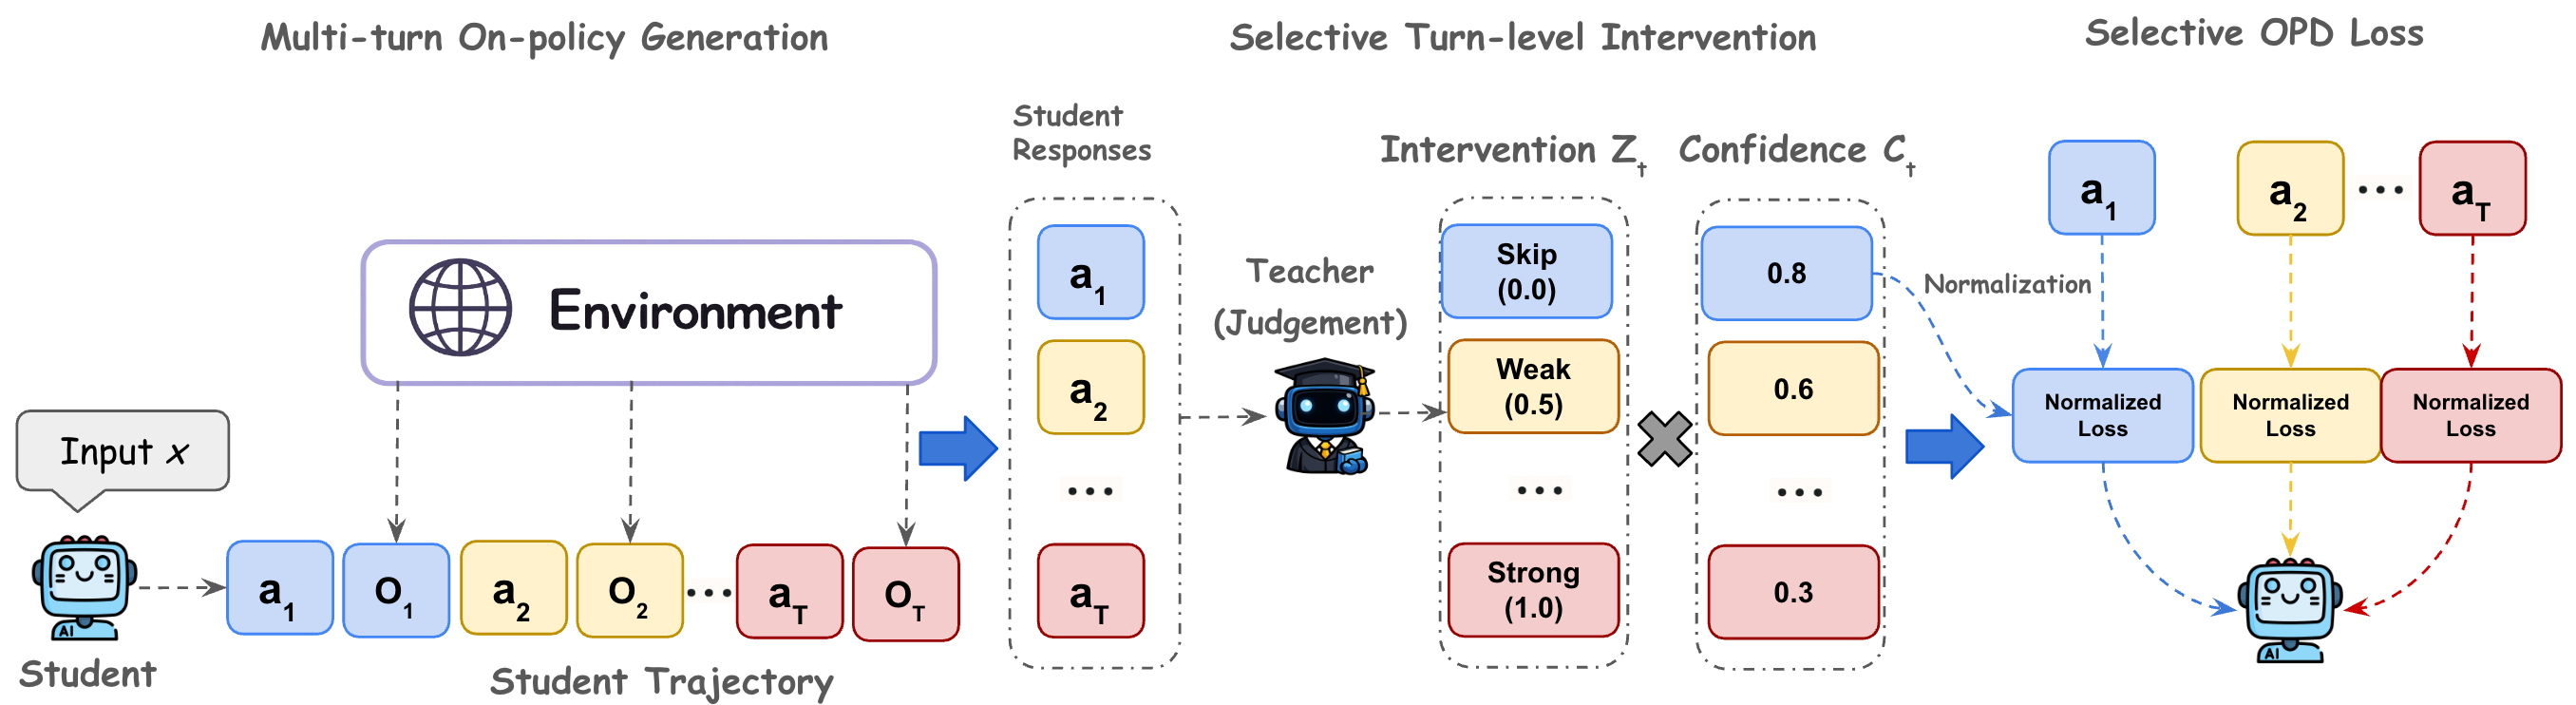
\includegraphics[width=\textwidth]{figure/diagram.png}
    \caption{
    Overview of \ours{}.
    %
    The student first performs multi-turn on-policy generation by interacting with the environment, producing a trajectory segmented into alternating actions and observations.
    %
    For each student turn, \ours{} uses environment feedback and teacher judgment to determine whether the response should be skipped or intervened on, and combines this intervention decision with the teacher confidence score.
    %
    The resulting selective weight modulates the OPD loss for each turn, so teacher supervision is applied more strongly when intervention is needed and the teacher signal is reliable.
    }
    \label{fig:our_framework}
\end{figure*}


\subsection{Preliminaries}

\paragraph{Multi-turn Agent Interaction.}
We consider a multi-turn agent interacting with an external environment over a sequence of action steps.
%
At turn $t$, the agent receives an observation $o_t$ and conditions on the full interaction history $h_t=(o_0,a_0,\ldots,o_{t-1},a_{t-1},o_t)$, where $a_i$ denotes the model response at turn $i$.
%
The response $a_t$ may include natural language reasoning, tool-use arguments, and an executable action.
%
After the executable part of $a_t$ is submitted to the environment, the environment returns the next observation $o_{t+1}\sim\mathcal{E}(\cdot\mid h_t,a_t)$.
%
A complete trajectory is $\tau=(h_0,a_0,\ldots,h_{T-1},a_{T-1})$, which terminates when a termination action is taken or when the maximum horizon $T$ is reached.
%
This dependency distinguishes multi-turn agent learning from single-turn generation: an early mistake can alter the environment state and affect all subsequent observations.

\paragraph{Multi-turn On-Policy Distillation.}
Let $\pi_\theta$ denote the student policy and $\pi_\phi$ denote the teacher policy.
%
In multi-turn OPD, trajectories are sampled from the student policy, i.e., $a_t\sim\pi_\theta(\cdot\mid h_t)$.
%
The teacher then provides supervision on these student-induced states.
%
We write the standard multi-turn OPD objective as
\begin{equation}
\label{eq:opd_objective}
\resizebox{0.96\columnwidth}{!}{$
\displaystyle
\mathcal{L}_{\mathrm{OPD}}
=
\mathbb{E}_{\tau\sim\pi_\theta}
\sum_{t=0}^{T-1}
\ell_{\mathrm{OPD}}(h_t),
\quad
\ell_{\mathrm{OPD}}(h_t)
=
D_{\mathrm{KL}}
\bigl(
\pi_\theta(\cdot\mid h_t)
\Vert
\pi_\phi(\cdot\mid h_t)
\bigr).
$}
\end{equation}
%
The student is therefore trained on its own state distribution, allowing the teacher to supervise states that arise from the student's behavior rather than only from ideal teacher-generated trajectories.

However, applying OPD uniformly to every turn in a multi-turn trajectory can be suboptimal.
%
Early student errors may alter future observations and push later histories away from the teacher's reliable state distribution, making subsequent supervision less dependable.
%
Meanwhile, token-level OPD can be brittle when teacher and student policies assign probability mass to different but semantically valid continuations, or when dense alignment reinforces local degeneracies such as repeated thoughts or actions.
%
These issues motivate a selective mechanism that decides when teacher distillation should be applied and how strongly the resulting signal should be trusted.

\subsection{\ours{}}
\label{sec:method}

The limitations of dense multi-turn OPD suggest that teacher supervision should be applied selectively rather than uniformly across all turns.
%
Standard OPD treats a student trajectory as a flat sequence of tokens and applies teacher distillation everywhere, which makes training sensitive to token-level mismatch even when the student response is semantically acceptable.
%
Multi-turn interaction provides a natural way to move beyond this flat token-level view: the trajectory is already segmented by environment feedback, where each turn produces a response $a_t$, receives an observation, and transitions to a new history $h_{t+1}$.
%
This turn structure allows the teacher to critique larger units of behavior and decide whether token-level distillation is needed for the current student response.

At the same time, teacher supervision should not be trusted uniformly across the trajectory.
%
Because student errors can compound over multiple turns, later histories may drift away from the teacher's reliable state distribution, making token-level supervision less dependable.
%
Motivated by these observations, and illustrated in \figref{fig:our_framework}, we propose \ours{}, a selective intervention framework for multi-turn OPD.
%
For each turn, \ours{} observes the environment feedback and uses teacher judgment to decide whether the current student response should be skipped or intervened on.
%
It then weights the token-level OPD objective by the teacher's predictive confidence, so supervision is strongest when intervention is needed and the teacher signal is reliable.
%
Finally, \ours{} applies vanilla-scale normalization to preserve the overall loss scale of standard OPD while retaining selective turn-level weighting.
%
The full training procedure is presented in Algorithm~\ref{alg:sl_opd} in \appref{sec:implementation_details}.

\subsection{Turn-Level Intervention}
\label{sec:method_intervention}

To obtain turn-level supervision without a task verifier, we introduce a discrete intervention label $z_t\in\{\textsc{Skip},\textsc{Weak},\textsc{Strong}\}$.
%
Each label is mapped to a scalar intervention weight:
\begin{equation}
\label{eq:intervention_weight}
i_t =
\begin{cases}
0, & z_t=\textsc{Skip},\\
\alpha, & z_t=\textsc{Weak},\\
1, & z_t=\textsc{Strong},
\end{cases}
\end{equation}
where $\alpha\in(0,1)$ controls the strength of weak intervention.
%
The \textsc{Skip} label suppresses OPD at the current turn, \textsc{Weak} applies partial teacher supervision, and \textsc{Strong} applies full teacher supervision.

We assign $z_t$ through a two-stage verifier-free procedure.
%
First, we inspect the environment feedback for deterministic interaction failures.
%
If the student response produces a clearly invalid transition, such as a failed tool call, missing executable action, or other environment-detectable execution failure, we directly set $z_t=\textsc{Strong}$ and $i_t=1$.
%
These cases do not require semantic judgment from the teacher, since the environment already indicates that the current response should be corrected.
%
For all remaining turns, where the response is executable but its quality is ambiguous, we query the teacher with an intervention-evaluation prompt.
%
Given the interaction history $h_t$, the student response $a_t$, and the available environment feedback, the teacher classifies the turn into exactly one of $\{\textsc{Skip},\textsc{Weak},\textsc{Strong}\}$.
%
Intuitively, \textsc{Skip} is used when the response is acceptable or when multiple strategies are plausible; \textsc{Weak} is used when the response may be suboptimal but the teacher is not fully certain; and \textsc{Strong} is used when the response is clearly detrimental and teacher correction is necessary.
%
Prompt details are provided in \appref{sec:appendix_prompts}.

\subsection{Teacher Confidence Weighting}

The intervention label determines whether teacher supervision is needed at a given turn.
%
However, even when intervention is needed, the teacher's token-level supervision may not always be reliable.
%
Due to compounding errors in multi-turn interaction, the student may enter histories that deviate from the teacher's reliable state distribution.
%
In such cases, the teacher may still recommend intervention, but its predictive distribution can be uncertain.
%
We therefore introduce a confidence score $c_t$ to measure how decisive the teacher is at turn $t$.

For each token position $j$ in the student response $a_t$, let $p^\star_{t,j}=\max_v\pi_\phi(v\mid h_t,a_{t,<j})$ denote the teacher's top-1 probability.
%
We define the turn-level confidence score and final selective weight as
\begin{equation}
\label{eq:confidence_weight}
c_t =
\frac{1}{|a_t|}
\sum_{j=1}^{|a_t|}
p^\star_{t,j},
\qquad
s_t = i_t c_t .
\end{equation}
%
A sharp teacher distribution yields a high $c_t$, indicating that the teacher is confident about the token-level supervision for this turn.
%
Conversely, a flat distribution yields a low $c_t$, indicating that the teacher itself is uncertain and that the resulting distillation signal should be weakened.
%
The same weight $s_t$ is applied uniformly to all token-level OPD terms within turn $t$.
%
Since $p^\star_{t,j}$ is obtained from the same teacher distribution used for the standard distillation loss, computing $c_t$ introduces no additional teacher forward passes beyond the intervention query.

\subsection{Vanilla-Scale Normalization}

The selective weight $s_t\in[0,1]$ controls how strongly teacher supervision is applied at turn $t$.
%
However, directly multiplying the OPD loss by $s_t$ also reduces the overall gradient magnitude relative to vanilla OPD.
%
This makes it difficult to distinguish the effect of selective supervision from the effect of training with a smaller effective learning rate.
%
To isolate the contribution of selective weighting, we normalize the loss scale within each batch.

Let $\ell_{\mathrm{OPD}}(h_t,a_t)$ denote the token-level OPD loss for turn $t$, and let $N$ denote the total number of student tokens in the trajectory or batch.
%
We define the normalized selective OPD objective as
\begin{equation}
\label{eq:selective_loss}
\begin{aligned}
\mathcal{L}_{\ours}
&=
Z\sum_{t}
s_t\ell_{\mathrm{OPD}}(h_t,a_t), \\
Z
&=
\frac{N}{
\max\!\left(
\sum_{t}s_t|a_t|,
\epsilon
\right)} .
\end{aligned}
\end{equation}
%
Here, $|a_t|$ is the number of student tokens in turn $t$, and $\epsilon$ is a small constant for numerical stability.
%
This normalization keeps the average effective token weight close to one, matching the scale of vanilla OPD while preserving the relative turn-level weighting induced by $s_t$.
%
As a result, \ours{} provides a verifier-free turn-level supervision policy that selectively reallocates teacher supervision without merely reducing the overall training signal.

\subsection{Analysis of Selective Weighting}
\label{sec:theory}

We provide an analysis to clarify the role of selective weighting in \ours{}.
%
Our goal is not to prove that the teacher intervention gate is always correct, but to formalize two intuitions: selective weights suppress noisy supervision from low-reliability turns, and the quality of selective OPD depends on how well its weights approximate an ideal intervention policy.
%
Let $\ell_t(\theta)$ denote the per-turn OPD loss at turn $t$, and let $s_t=i_tc_t\in[0,1]$ be the selective weight.
%
The normalized objective follows \eqref{eq:selective_loss}, with $\ell_{\mathrm{OPD}}(h_t,a_t)$ replaced by $\ell_t(\theta)$.

\paragraph{Selective suppression of noisy supervision.}
Assume that the observed per-turn OPD loss decomposes as $\ell_t(\theta)=\ell_t^\star(\theta)+\xi_t$, where $\ell_t^\star$ is the ideal supervision loss and $\xi_t$ is zero-mean noise caused by teacher uncertainty, token-level mismatch, or off-distribution histories.
%
Assume $\mathrm{Var}[\xi_t]\leq\sigma_t^2$.
%
For a fixed batch, define the normalized effective weight as $\widetilde{s}_t=Zs_t$.

\begin{proposition}[Relative Suppression of Noisy Supervision]
\label{prop:relative_suppression}
The variance contribution of turn $t$ to the noisy component of the normalized selective objective is bounded by
\begin{equation}
\label{eq:noise_bound}
\mathrm{Var}[\widetilde{s}_t\xi_t]
\leq
\widetilde{s}_t^2\sigma_t^2 .
\end{equation}
Moreover, if two turns $p$ and $q$ satisfy $s_p\leq\gamma s_q$ for some $\gamma<1$, then their per-unit-noise contributions satisfy $\widetilde{s}_p^2/\widetilde{s}_q^2\leq\gamma^2$.
\end{proposition}

This proposition does not claim that the total variance of \ours{} is always smaller than that of vanilla OPD.
%
Because vanilla-scale normalization may produce $Z>1$, the absolute variance of the normalized objective can increase in some batches.
%
Instead, the result shows that the relative suppression induced by $s_t$ is preserved after normalization.
%
When the intervention mechanism assigns smaller weights to unnecessary or unreliable turns, their noisy teacher gradients are reduced relative to turns where intervention is needed and the teacher signal is confident.
%
The proof is provided in \appref{sec:appendix_theory}.

\paragraph{Connection to oracle intervention.}
An ideal selective OPD objective would supervise exactly the turns where teacher correction is useful.
%
Let $m_t^\star\in\{0,1\}$ denote this unobserved oracle intervention indicator, where $m_t^\star=1$ means that turn $t$ should receive teacher supervision and $m_t^\star=0$ means that it should be skipped.
%
The oracle objective is $\mathcal{L}_{\mathrm{oracle}}(\theta)=\sum_{t=0}^{T-1}m_t^\star\ell_t(\theta)$.
%
Our method replaces this binary oracle mask with the verifier-free soft weight $s_t=i_tc_t$.

\begin{proposition}[Approximation Error of Selective Intervention]
\label{prop:oracle_approx}
If the per-turn loss is bounded as $0\leq\ell_t(\theta)\leq B$, then
\begin{equation}
\label{eq:oracle_bound}
\left|
\sum_{t=0}^{T-1}
(s_t-m_t^\star)\ell_t(\theta)
\right|
\leq
B\sum_{t=0}^{T-1}
|s_t-m_t^\star| .
\end{equation}
\end{proposition}

This bound is not a guarantee that \ours{} recovers the oracle mask.
%
Rather, it makes explicit that the gap to oracle selective supervision is controlled by the quality of the intervention weights.
%
In \ours{}, deterministic environment failures provide high-precision positive intervention signals, teacher judgment approximates the oracle decision for executable but ambiguous turns, and teacher confidence softens the weight when token-level supervision is uncertain.
%
The proof is provided in \appref{sec:appendix_theory}.
\section{Experiments}
\label{sec:experiments}

\subsection{Experiment Setup}
\label{sec:setup}

\paragraph{Models.}
Following prior work on multi-turn on-policy distillation, we use teacher and student models from the same model family to reduce confounding effects from tokenizer, architecture, and instruction-format mismatch. Specifically, we use Qwen3-32B and Qwen3-8B as teacher models, and Qwen3-0.6B and Qwen3-1.7B as student models \citep{yang2025qwen3}. This yields multiple teacher--student pairs with different capacity gaps, allowing us to evaluate whether \ours{} remains effective across both large-gap and moderate-gap distillation settings.

\paragraph{Datasets and Evaluation.}
We evaluate \ours{} on three multi-turn agent benchmarks: ALFWorld \citep{shridhar2020alfworld}, ScienceWorld \citep{wang2022scienceworld}, and SearchQA \citep{jin2025search}. These benchmarks cover embodied interaction, scientific task solving, and search-based question answering, respectively, allowing us to assess the effectiveness of selective intervention across different forms of multi-turn decision making.

For ALFWorld, we report success rate (SR) on both the seen and unseen splits. For ScienceWorld, we report success rate (SR) and the mean score on the test set. For SearchQA, we report exact match (EM) across different question-answering datasets. Detailed definitions of the evaluation metrics are provided in \appref{sec:implementation_details}.

\paragraph{Baselines.}
We compare \ours{} with four main baselines: off-policy SFT, vanilla OPD, TCOD (F2B) \citep{wang2026tcod}, and Entropy-Aware OPD \citep{jin2026entropy}. TCOD-F2B stabilizes multi-turn OPD through a forward-to-backward temporal curriculum, and Entropy-Aware OPD augments OPD with entropy-gated KL loss originally designed for single-turn distillation. 
%
Since \ours{} uses one additional teacher query to obtain the turn-level intervention label, it introduces extra inference cost compared with vanilla OPD.
%
In practice, this overhead is limited because most prompt tokens are shared with the rollout context and can be cached, while the intervention output is only a short label.
%
Nevertheless, to control for the additional teacher-query budget, we include a compute-matched baseline, vanilla OPD with two rollouts, where both the student and teacher are queried twice during OPD data collection.

\paragraph{Training Details.}
We implement OPD with a fully asynchronous rollouter--trainer pipeline. Unless otherwise specified, all methods are trained for one epoch with learning rate $1\times10^{-6}$ and rollout number 1. We use student temperature $0.4$, teacher temperature $0.0$, top-$p=1.0$, and top-$k=-1$ as the default setup. For \ours{}, we set the weak-intervention coefficient to $\alpha=0.5$. We analyze the sensitivity to this choice in \secref{sec:sensitivity_analysis}. Additional implementation details are provided in \appref{sec:implementation_details}.


\subsection{Main Results}
\label{sec:result_analysis}

\begin{table*}[t]
\centering
\caption{Main results on ALFWorld. We report success rate (SR) and average number of turns on both seen and unseen splits. Best SR among distillation methods for each student--teacher setup is in \textbf{bold}, and the second-best SR is \underline{underlined}.}
\label{tab:main_results_alfworld}
\resizebox{0.95\textwidth}{!}{%
\begin{tabular}{lllcccc}
\toprule
\textbf{Student Model} & \textbf{Teacher Model} & \textbf{Method}
& \textbf{Seen SR} & \textbf{Seen Turns}
& \textbf{Unseen SR} & \textbf{Unseen Turns} \\
\midrule
\multicolumn{7}{c}{\textit{Reference Models (Base Inference)}} \\
\midrule
Qwen3-0.6B & -- & Base & 1.43 & 29.65 & 0.75 & 29.82 \\
Qwen3-1.7B & -- & Base & 25.71 & 24.63 & 26.12 & 24.72 \\
-- & Qwen3-8B & Base & 61.43 & 17.95 & 67.16 & 17.24 \\
-- & Qwen3-32B & Base & 57.14 & 18.94 & 69.40 & 18.21 \\
\midrule
\multicolumn{7}{c}{\textit{Student: Qwen3-0.6B, Teacher: Qwen3-8B}} \\
\midrule
\multirow{6}{*}{Qwen3-0.6B} & \multirow{6}{*}{Qwen3-8B} & SFT & 2.86 & 29.32 & 4.48 & 28.87 \\
 & & OPD & 55.00 & 18.53 & 56.72 & 20.30 \\
 & & OPD (rollout 2) & \underline{56.43} & 18.76 & 59.70 & 20.31 \\
 & & Entropy-Aware OPD & 54.26 & 18.12 & 54.48 & 20.75 \\
 & & TCOD-F2B & \underline{56.43} & 18.51 & \underline{61.19} & 18.82 \\
 & & \ours{} & \textbf{57.86} & 18.46 & \textbf{61.94} & 18.89 \\
\midrule
\multicolumn{7}{c}{\textit{Student: Qwen3-1.7B, Teacher: Qwen3-8B}} \\
\midrule
\multirow{6}{*}{Qwen3-1.7B} & \multirow{6}{*}{Qwen3-8B} & SFT & 25.00 & 24.58 & 26.12 & 24.54 \\
 & & OPD & 60.00 & 17.80 & 61.94 & 17.67 \\
 & & OPD (rollout 2) & 63.00 & 17.51 & 64.93 & 17.87 \\
 & & Entropy-Aware OPD & 63.57 & 17.28 & \underline{65.67} & 18.20 \\
 & & TCOD-F2B & \textbf{64.29} & 17.65 & 58.21 & 19.16 \\
 & & \ours{} & \textbf{64.29} & 18.14 & \textbf{70.15} & 17.86 \\
\midrule
\multicolumn{7}{c}{\textit{Student: Qwen3-0.6B, Teacher: Qwen3-32B}} \\
\midrule
\multirow{5}{*}{Qwen3-0.6B} & \multirow{5}{*}{Qwen3-32B} & OPD & 53.57 & 19.49 & 68.66 & 18.65 \\
 & & OPD (rollout 2) & 52.14 & 20.28 & \underline{70.37} & 18.21 \\
 & & Entropy-Aware OPD & 48.57 & 20.87 & 68.13 & 18.28 \\
 & & TCOD-F2B & \textbf{54.29} & 20.18 & 67.91 & 19.26 \\
 & & \ours{} & \textbf{54.29} & 19.85 & \textbf{70.90} & 17.98 \\
\midrule
\multicolumn{7}{c}{\textit{Student: Qwen3-1.7B, Teacher: Qwen3-32B}} \\
\midrule
\multirow{5}{*}{Qwen3-1.7B} & \multirow{5}{*}{Qwen3-32B} & OPD & 58.57 & 18.89 & \underline{74.85} & 17.16 \\
 & & OPD (rollout 2) & \underline{62.14} & 18.17 & 72.39 & 18.37 \\
 & & Entropy-Aware OPD & 60.00 & 18.80 & \textbf{79.10} & 16.75 \\
 & & TCOD-F2B & 57.14 & 19.42 & 73.13 & 17.87 \\
 & & \ours{} & \textbf{62.82} & 18.75 & 73.88 & 17.57 \\
\bottomrule
\end{tabular}%
}
\end{table*}

We present the main results on ALFWorld, ScienceWorld, and SearchQA in \tabref{tab:main_results_alfworld}, \tabref{tab:main_results_scienceworld}, and \tabref{tab:main_results_searchqa} in \appref{sec:supplementary_results}, respectively.

\paragraph{Improvements over Base Models, SFT, and Vanilla OPD.}
Across all three benchmarks, \ours{} substantially improves over base student models and off-policy SFT. 
%
On ALFWorld, Qwen3-0.6B improves from $1.43/0.75$ SR on seen/unseen splits to $57.86/61.94$ with a Qwen3-8B teacher, while reducing the average number of turns from nearly $30$ to about $18$--$19$. 
%
Compared with vanilla OPD, \ours{} further improves Qwen3-0.6B from $55.00$ to $57.86$ seen SR and from $56.72$ to $61.94$ unseen SR, while improving Qwen3-1.7B unseen SR from $61.94$ to $70.15$. 
%
These gains are not merely due to extra teacher queries, as \ours{} also outperforms the compute-matched OPD rollout-$2$ baseline in most ALFWorld settings, with comparable or fewer turns on the unseen split.

\paragraph{Comparison with Strong OPD Variants.}
Compared with TCOD-F2B and Entropy-Aware OPD, \ours{} is strongest on ALFWorld and remains competitive on ScienceWorld and SearchQA. 
%
On ALFWorld, \ours{} achieves the best unseen SR in three out of four student--teacher settings and ties for the best seen SR in two settings, while generally maintaining similar turn efficiency to the strongest baselines. 
%
On SearchQA, \ours{} obtains the best average EM for Qwen3-1.7B distilled from Qwen3-8B, improving over OPD from $30.09$ to $30.77$. 
%
On ScienceWorld, \ours{} achieves the best SR for Qwen3-1.7B with both Qwen3-8B and Qwen3-32B teachers, and improves the Qwen3-0.6B mean score with Qwen3-8B from $-12.88$ under OPD to $+3.89$, although this comes with a higher average number of turns, suggesting more sustained task exploration.

\paragraph{Effects of Student and Teacher Scale.}
The benefits of \ours{} are more consistent for the larger Qwen3-1.7B student, which achieves strong gains on ALFWorld, the best average SearchQA result, and the best ScienceWorld SR across both teacher settings. 
%
For Qwen3-0.6B, OPD already provides large gains over SFT and base inference, while \ours{} further improves ALFWorld generalization but shows more task-dependent effects on ScienceWorld and SearchQA. 
%
Increasing teacher size is not uniformly beneficial, suggesting that stronger teacher signals are not automatically more reliable when applied densely and that adaptive weighting is important for multi-turn OPD.


\begin{figure*}[t]
    \centering
    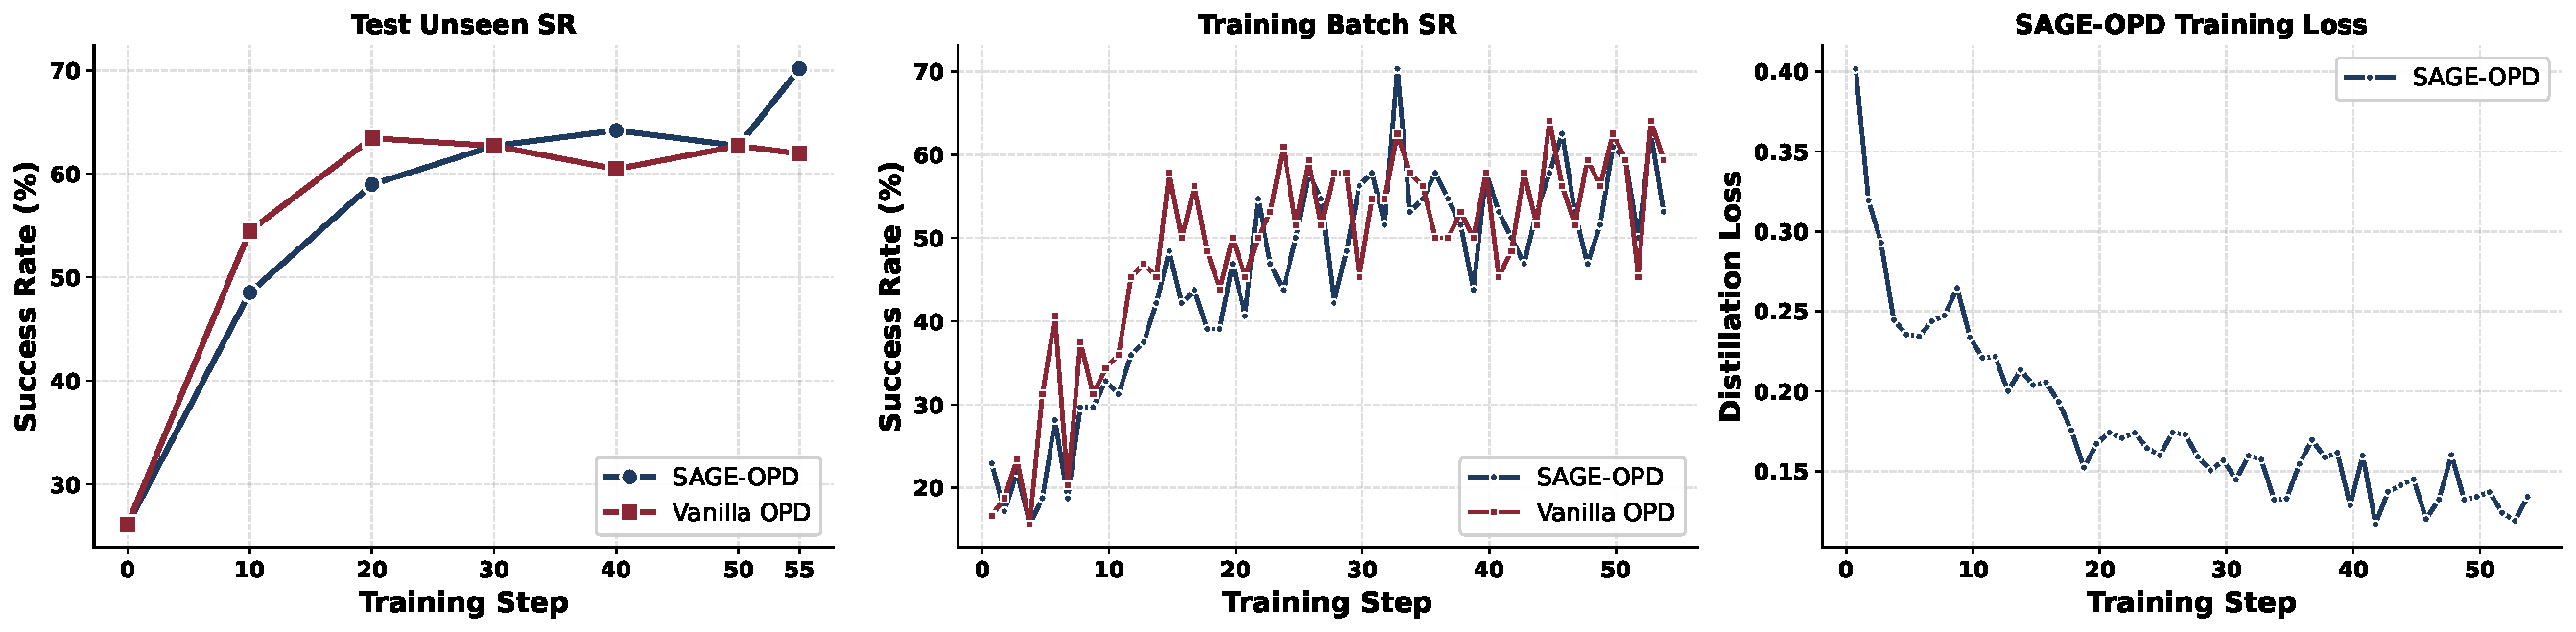
\includegraphics[width=\textwidth]{figure/alfworld_sl_opd_vs_vanilla.pdf}
    \caption{Training dynamics on ALFWorld comparing \ours{} with vanilla OPD. Left: test unseen success rate during training. Middle: training-batch success rate. Right: training loss of \ours{}.}
    \label{fig:training_dynamics}
\end{figure*}

\subsection{Training Dynamics}

\figref{fig:training_dynamics} compares the training dynamics of \ours{} and vanilla OPD on ALFWorld. 
%
On the unseen test split, both methods improve rapidly in the early stage, but vanilla OPD saturates after roughly 20--30 training steps, fluctuating around $60$--$63\%$ SR. 
%
In contrast, \ours{} continues to improve in the later stage and reaches $70.15\%$ unseen SR by the end of training. 
%
This suggests that selective intervention does not merely accelerate early learning, but also helps maintain useful teacher supervision after vanilla dense OPD begins to plateau.

The training-batch success rate shows a similar trend: both methods improve throughout training, while \ours{} remains competitive with vanilla OPD despite applying supervision selectively rather than uniformly. 
%
The right panel further shows that the \ours{} distillation loss decreases steadily over training, indicating stable optimization under the intervention-weighted objective. 
%
Together, these dynamics support our hypothesis that selectively reallocating teacher supervision can improve generalization while preserving stable on-policy training.
\section{Analysis}
\label{sec:analysis}

\paragraph{Intervention behavior.}
We further analyze the behavior of the intervention gate in \figref{fig:intervention_analysis} in \appref{sec:appendix_intervention_analysis}.
%
According to this figure, \ours{} assigns more \textsc{Skip} labels and fewer \textsc{Weak}/\textsc{Strong} labels as training progresses, indicating that the student gradually produces more acceptable actions and requires less teacher correction.
%
Across turn positions, \textsc{Skip} remains the dominant label but becomes less frequent in later turns, while deterministic failures increase, suggesting that response quality becomes harder to maintain as interaction histories grow longer.
%
These trends support the motivation for selective multi-turn OPD: \ours{} does not uniformly downweight late turns, but distinguishes acceptable behavior, uncertain behavior, and clear execution failures. Detailed label distributions and analysis are provided in \appref{sec:appendix_intervention_analysis}.

\paragraph{Ablation study.}
We conduct incremental ablations on ALFWorld to isolate the contribution of each component in \ours{}.
%
The \textit{Intervention-only} variant already performs strongly, showing that teacher-judged turn-level intervention can identify useful correction points without requiring a task-level verifier.
%
Adding teacher confidence gives \ours{}-NoNorm, which improves some settings but can also reduce unseen generalization when selective weights shrink the effective training signal.
%
The full \ours{} objective addresses this issue with vanilla-scale normalization, improving unseen SR from $64.93$ to $70.15$ for Qwen3-1.7B distilled from Qwen3-8B and from $69.40$ to $70.90$ for Qwen3-0.6B distilled from Qwen3-32B.
%
Overall, intervention weighting, teacher confidence, and loss-scale normalization play complementary roles in selective multi-turn OPD.
%
Full ablation results are provided in \appref{sec:appendix_ablation}.

\paragraph{Sensitivity Analysis}
\label{sec:sensitivity_analysis}

\begin{table}[t]
\centering
\caption{Sensitivity analysis on ALFWorld using Qwen3-8B as teacher and Qwen3-1.7B as student. The default configuration uses $\alpha=0.5$, teacher temperature $0.0$, and vanilla-scale normalization over all student tokens.}
\label{tab:sensitivity}
\resizebox{\columnwidth}{!}{%
\begin{tabular}{llcccc}
\toprule
\textbf{Type} & \textbf{Setting} & \textbf{Seen SR} & \textbf{Unseen SR} & \textbf{Seen Turns} & \textbf{Unseen Turns} \\
\midrule
\multirow{4}{*}{$\alpha$}
& $0.3$ & 63.57 & 67.16 & 17.34 & 16.78 \\
& $0.5$ \;(\textit{default}) & \textbf{64.29} & \textbf{70.15} & 18.14 & 17.86 \\
& $0.7$ & 57.86 & 66.42 & 18.86 & 18.47 \\
& $1.0$ & 58.57 & 61.94 & 19.31 & 19.02 \\
\midrule
\multirow{5}{*}{Teacher temp.}
& $0.0$ \;(\textit{default}) & \textbf{64.29} & \textbf{70.15} & 18.14 & 17.86 \\
& $0.3$ & 60.00 & 62.69 & 18.61 & 18.35 \\
& $0.7$ & 60.71 & 65.67 & 18.77 & 18.34 \\
& $1.0$ & 60.71 & 63.43 & 18.24 & 18.11 \\
& $1.5$ & 57.86 & 63.43 & 19.24 & 18.74 \\
\midrule
Normalization
& Active-token norm. & 62.14 & 68.66 & 18.41 & \textbf{17.46} \\
\bottomrule
\end{tabular}%
}
\end{table}

We analyze the sensitivity of \ours{} on ALFWorld using Qwen3-8B as teacher and Qwen3-1.7B as student.
%
As shown in \tabref{tab:sensitivity}, the default weak-intervention weight $\alpha=0.5$ achieves the best seen and unseen SR.
%
A smaller value, $\alpha=0.3$, remains competitive but underperforms on the unseen split, suggesting that weak interventions still provide useful supervision.
%
Larger values, such as $\alpha=0.7$ and $\alpha=1.0$, degrade performance and increase the average number of turns, indicating that treating weak interventions too similarly to strong interventions can over-regularize the student.
%
We also vary the teacher temperature used for confidence estimation.
%
The default deterministic setting, temperature $0.0$, performs best, while higher temperatures consistently reduce success rate, likely because the confidence score becomes less stable.
%
Finally, an alternative normalization that counts only active, non-skipped tokens remains competitive with $68.66\%$ unseen SR, but underperforms the default vanilla-scale normalization at $70.15\%$.
%
Overall, these results support using a moderate weak-intervention weight, deterministic teacher confidence, and normalization over all student tokens as the default configuration.


\section{Conclusion}

We introduced \ours{}, a verifier-free selective intervention framework for multi-turn OPD. Instead of applying teacher supervision uniformly across all turns, \ours{} first estimates whether each student response requires intervention and then weights token-level distillation by teacher confidence, addressing both compounding errors across interaction steps and brittle token-level supervision in ambiguous states. Experiments on ALFWorld, ScienceWorld, and SearchQA show that \ours{} improves over base students, off-policy SFT, and vanilla OPD while remaining competitive with strong OPD variants. Ablation and training-dynamics analyses further demonstrate that intervention labels, teacher confidence weighting, and vanilla-scale normalization provide complementary benefits. Overall, our results suggest that effective multi-turn OPD should be on-policy but not necessarily dense: teacher supervision should be selectively allocated to turns where intervention is necessary and reliable.



\section{Limitations}
\label{sec:limitations}

Although \ours{} relies on teacher judgment for turn-level intervention, we take several steps to validate that the intervention mechanism is not overly brittle.
%
We evaluate across different student and teacher sizes, multiple multi-turn agent benchmarks, and conduct case studies showing that the intervention labels distinguish acceptable, ambiguous, harmful, and deterministic-failure turns.
%
We also vary the teacher temperature to test the sensitivity of confidence estimation, finding that deterministic teacher confidence provides the strongest performance while higher temperatures degrade results.
%
Nevertheless, the intervention labels are still produced by the teacher rather than by an external oracle.
%
If the teacher systematically misjudges the student's behavior, \ours{} may skip harmful actions or over-correct acceptable alternatives.
%
Similarly, the confidence score is based on the sharpness of the teacher's token-level distribution, which is only a proxy for supervision reliability; a confident distribution does not always imply semantic correctness, especially on severely off-distribution histories.

Our experiments focus on text-based multi-turn agent benchmarks, including embodied interaction, scientific task solving, and search-based question answering.
%
While these environments cover diverse forms of interaction, they are still more structured than many real-world tool-use and software-engineering settings.
%
Extending \ours{} to broader high-latency or open-ended agent domains may require task-specific intervention prompts, richer environment feedback, or different deterministic-failure detectors.
%
In addition, \ours{} introduces an extra teacher query for turn-level intervention.
%
In practice, this overhead is mitigated because most input tokens can be cached and the teacher only outputs a short intervention label, but it still increases data-collection cost compared with vanilla OPD.
%
Reducing this overhead, for example by training a lightweight intervention model or reusing cached teacher judgments, is an important direction for future work.

\section{Ethical Considerations}
We utilized GPT-based models \citep{openai2023gpt4} solely for language polishing and proofreading.
%
This work studies training methods for multi-turn LLM agents using public benchmark environments and does not introduce new datasets containing personal or sensitive information.
%
\ours{} relies on teacher judgments, so biases or unsafe preferences in the teacher model may be propagated to the student.
%
Practical deployment should therefore include appropriate action validation, safety constraints, logging, and human oversight.


\bibliography{custom}

\appendix

\appendix
\section*{Appendix}

\section{Related Work}
\label{sec:related_work}

\paragraph{Multi-Turn LLM Agents.}
Recent LLM agents extend language models from single-turn text generation to interactive decision making, where the model repeatedly observes an environment, produces an action or tool call, and receives new feedback \citep{yao2022react, yang2024swe, chan2025mle}. These multi-turn agents have been studied in embodied simulators \citep{shridhar2020alfworld}, web navigation \citep{gur2024real, team2025tongyi}, tool use \citep{yao2024tau}, and search-based question answering \citep{jin2025search}. Compared with single-turn tasks, multi-turn agent learning is more challenging because the model must maintain a long interaction history, reason over partially observable states, and recover from its own previous mistakes. An early suboptimal action can change the future observation stream, causing errors to compound across the trajectory \citep{zhang2025agentracer}.

To improve multi-turn agent performance, prior work has mainly explored two training paradigms. The first is multi-turn SFT \citep{teng2024fine, li2025beyond}, which decomposes teacher trajectories into turn-level training examples and trains the model to imitate them. This can improve formatting and local action prediction, but it remains off-policy: the student is optimized on teacher-generated states rather than the histories induced by its own behavior. The second is reinforcement learning with verifiable rewards (RLVR) \citep{shao2024deepseekmath}, where the agent receives reward from the final environment outcome \citep{deepswe2025, wei2025webagent}. While this directly optimizes task success, it typically requires an external verifier or environment-defined reward signal, and the resulting reward is often sparse relative to the long sequence of student-generated turns, making credit assignment difficult~\citep{wang2026openclaw}. These limitations motivate on-policy distillation methods that can provide teacher supervision on student-induced trajectories while avoiding the sparsity of pure outcome-based reward learning.

\paragraph{On-Policy Distillation and Multi-Turn Limitations.}
To mitigate the exposure bias of offline imitation, OPD shifts supervision from teacher-generated trajectories to the student's own generated distribution \citep{agarwal2024policy, lu2025onpolicydistillation}. In OPD, the student first samples trajectories under its current policy, and the teacher then provides token-level feedback on the resulting student-induced states. This aligns training with inference-time behavior and allows the student to learn from states that arise from its own decisions, rather than only from expert demonstrations \citep{zhao2026self, he2026self, hubotter2026reinforcement}.

Despite this advantage, recent analyses have revealed that the token-level logit signal underlying standard OPD is surprisingly brittle. This brittleness is further amplified in multi-turn settings, where local token-level mismatches can compound across turns. First, OPD relies on a narrow token-level overlap between the teacher's and student's plausible next-token distributions \citep{li2026rethinking}. When multiple continuations are semantically valid, dense token-level alignment can over-penalize acceptable alternatives. Second, OPD can reinforce degenerate local patterns when repeated or low-quality prefixes accidentally receive favorable token-level gradients \citep{luo2026demystifying}; in multi-turn agents, this may manifest as repeated thoughts or repeated actions across consecutive turns. Third, multi-turn interaction amplifies distribution shift through compounding errors: student thoughts or actions can push the environment history outside the teacher's effective state distribution, making later teacher supervision less reliable \citep{wang2026tcod, li2025beyond}.

A concurrent line of work, TCOD, addresses this instability by controlling the trajectory depth and gradually expanding the student-controlled horizon through a temporal curriculum \citep{wang2026tcod}. In contrast, \ours{} does not rely on a manually designed curriculum over turn depth. Instead, we delegate the intervention decision to the teacher: for each turn, the teacher determines whether supervision should be skipped, weakly applied, or strongly applied. To further account for compounding errors that may move the student into states where the teacher is less reliable, \ours{} weights the token-level OPD signal by the teacher's predictive confidence. Thus, rather than deciding \emph{how long} to apply OPD, \ours{} decides \emph{where} OPD should be applied and how strongly it should be trusted.

\section{Proofs for Selective Weighting Analysis}
\label{sec:appendix_theory}

\begin{proof}[Proof of Proposition~\ref{prop:relative_suppression}]
For a fixed batch, the noisy component of the normalized selective objective is
\[
    Z\sum_{t=0}^{T-1}s_t\xi_t
    =
    \sum_{t=0}^{T-1}\widetilde{s}_t\xi_t,
\]
where $\widetilde{s}_t=Zs_t$.
%
The variance contribution of turn $t$ is
\[
    \mathrm{Var}[\widetilde{s}_t\xi_t]
    =
    \widetilde{s}_t^2\mathrm{Var}[\xi_t]
    \leq
    \widetilde{s}_t^2\sigma_t^2,
\]
which proves \eqref{eq:noise_bound}.
%
For any two turns $p$ and $q$, the shared normalization factor cancels:
\[
    \frac{\widetilde{s}_p^2}{\widetilde{s}_q^2}
    =
    \frac{Z^2s_p^2}{Z^2s_q^2}
    =
    \frac{s_p^2}{s_q^2}.
\]
%
Therefore, if $s_p\leq\gamma s_q$ for $\gamma<1$, then $\widetilde{s}_p^2/\widetilde{s}_q^2\leq\gamma^2$.
\end{proof}

\begin{proof}[Proof of Proposition~\ref{prop:oracle_approx}]
By the triangle inequality and the bounded-loss assumption,
\[
\begin{aligned}
\left|
\sum_{t=0}^{T-1}
(s_t-m_t^\star)\ell_t(\theta)
\right|
&\leq
\sum_{t=0}^{T-1}
|s_t-m_t^\star|\,|\ell_t(\theta)| \\
&\leq
B\sum_{t=0}^{T-1}
|s_t-m_t^\star|.
\end{aligned}
\]
%
This proves \eqref{eq:oracle_bound}.
\end{proof}

\section{Implementation Details}
\label{sec:implementation_details}


We implement \ours{} and all baselines on top of the \texttt{verl} fully-asynchronous pipeline, using a decoupled rollouter--trainer architecture with a staleness-bounded queue. We set \texttt{trigger\_parameter\_sync\_step} to $4$ and \texttt{staleness\_threshold} to $0.5$. We use AdamW with a learning rate $10^{-6}$, weight decay $0.1$, response length $4096$, rollout number $n=1$, global batch size 64, and epoch number 1. 

The maximum number of turns is $30$ for ALFWorld and ScienceWorld and $16$ for SearchQA.
%
The maximum generation length is $4096$ tokens per turn.
%
We use student temperature $0.4$, teacher temperature $0.0$, top-$p=1.0$, and top-$k=-1$ as the default setup.
%
All evaluations use the ReAct prompt format with full chat history, no sliding window, thinking mode disabled, and \texttt{</action>} as the stop string.
%
For SearchQA, the agent is allowed at most $8$ search calls per episode and retrieves the top $3$ documents from a Wikipedia-2018 index using dense E5 retrieval with FAISS-Flat.
%
We evaluate on the standard ALFWorld valid-seen and valid-unseen splits, the ScienceWorld test set with $30$ task types and $5$ variations per task, and capped SearchQA splits with up to $500$ questions per split except Bamboogle, which contains $125$ questions.


For agentic OPD baselines, we keep the OPD backbone fixed and modify only the per-token or per-turn weighting scheme. TCOD-F2B truncates each rollout after
\begin{equation}
    k(n) = \min\left(k_{\mathrm{start}} + \frac{n}{\eta}, T\right)
\end{equation}
assistant turns. We set $k_{\mathrm{start}}=1$ and $\eta=1$. The maximum horizon is $T=30$ for ALFWorld and ScienceWorld, and $T=16$ for SearchQA, so the curriculum reaches the cap within one epoch. Entropy-Aware OPD scales the per-token weight by
\begin{equation}
    1 + \alpha_e \cdot \mathbf{1}
    \left[
    H_{\phi}(\cdot \mid h_t,a_{t,<j}) > \tau_e
    \right],
\end{equation}
where $H_{\phi}$ is estimated from the cached top-$K$ teacher distribution. We use $\tau_e=0.8$ and $\alpha_e=1.0$.

For \ours{}, the selective weight is defined as
\begin{equation}
    s_t = i_t \cdot c_t.
\end{equation}
The default per-turn intervention weight $i_t \in \{0,0.5,1\}$ ($\alpha=0.5$) is obtained from one short teacher query per assistant turn, using maximum generation length $1028$ and default temperature $0.0$. If the teacher output is unparseable, we conservatively fall back to $i_t=1$. We also retain the deterministic-failure short circuit: if the student turn is empty, unparseable, or violates the required action schema, we directly set $i_t=1$ without relying on the teacher intervention query.

We use the training split of each benchmark for training. For SearchQA \citep{jin2025search}, we randomly sample 10K examples from the training split as the training subset.

\paragraph{Evaluation Metrics.}
We use benchmark-specific metrics following the standard evaluation protocols.
%
For ALFWorld, we report success rate (SR) on the valid-seen and valid-unseen splits, where an episode is counted as successful if the environment returns \texttt{info["won"] = True} within the turn budget.
%
For ScienceWorld, we report both SR and mean score.
%
SR counts episodes whose cumulative score reaches $100$, while mean score averages the environment-provided cumulative reward over episodes.
%
Since ScienceWorld provides partial credit and small models rarely solve tasks end-to-end, mean score is a more sensitive measure of partial progress and catastrophic failures.
%
For SearchQA, we report exact match (EM), where the final answer is counted as correct if its normalized string matches any reference answer.
%
We follow the SearchR1 normalization protocol, which lowercases text, removes punctuation and articles, and collapses whitespace.
%
For SearchQA, we report EM on each evaluation split and macro-average across NQ, TriviaQA, PopQA, HotpotQA, 2WikiMultiHopQA, Musique, and Bamboogle.
%
We also report average number of turns for ALFWorld and ScienceWorld, and average search/turn statistics for SearchQA as auxiliary efficiency metrics.


\section{Supplementary Results}
\label{sec:supplementary_results}


\subsection{Intervention Analysis}
\label{sec:appendix_intervention_analysis}

\begin{figure*}[t]
    \centering
    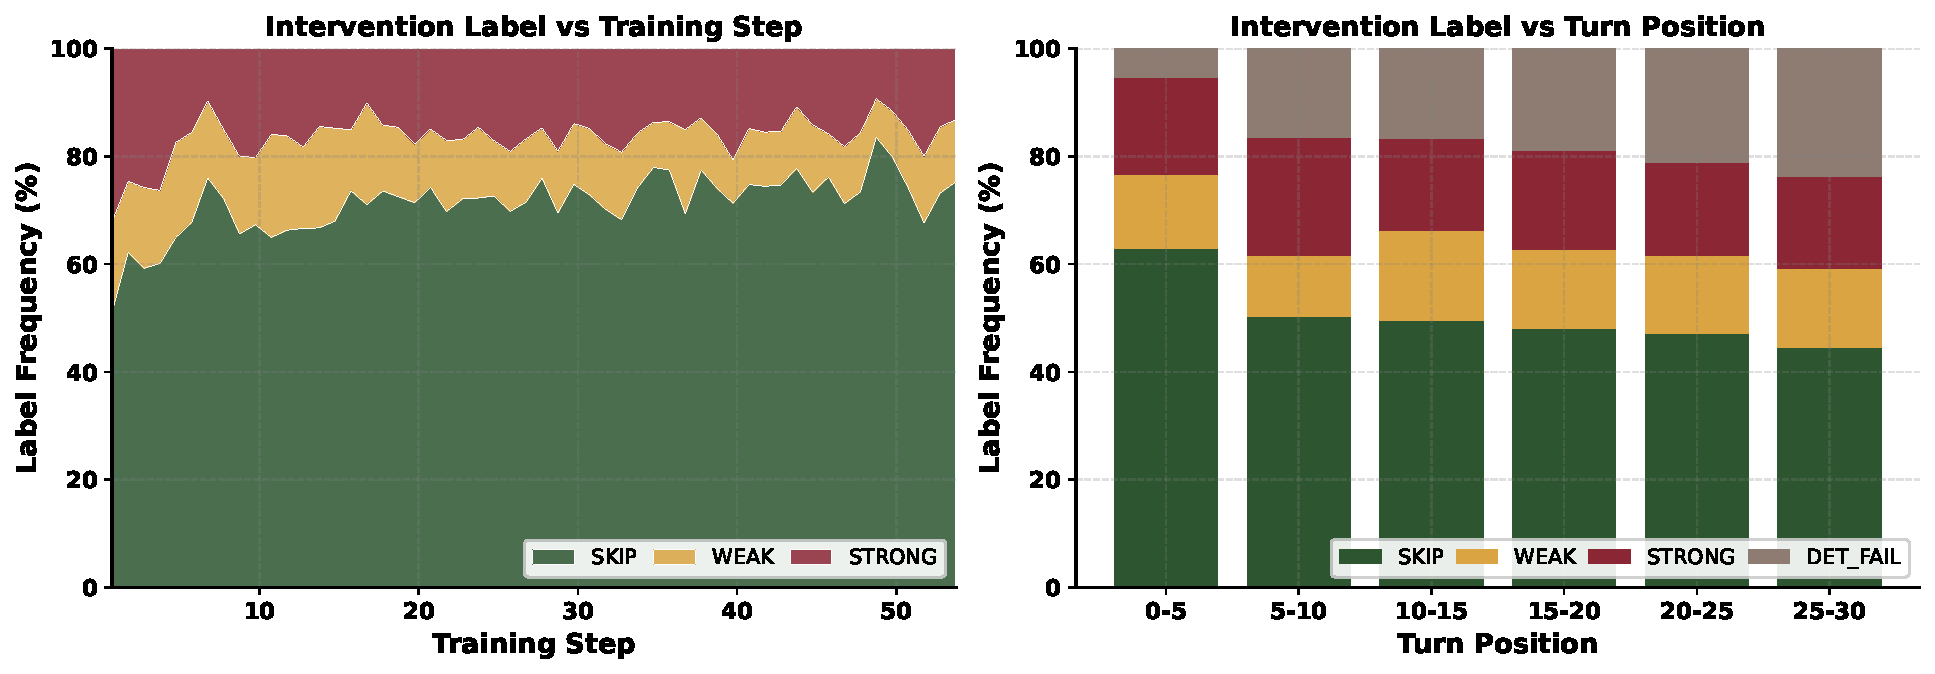
\includegraphics[width=0.9\textwidth]{figure/alfworld_slopd_intervention.pdf}
    \caption{Intervention label distribution of \ours{} on ALFWorld. Left: label frequency across training steps. Right: label frequency across turn positions. \textsc{Det-Fail} denotes deterministic failures detected before teacher intervention, such as malformed actions, failed tool calls, missing executable actions, or environment-reported execution failures.}
    \label{fig:intervention_analysis}
\end{figure*}

\figref{fig:intervention_analysis} analyzes the intervention labels produced by \ours{} across training steps and turn positions.
%
In addition to the teacher-assigned labels \textsc{Skip}, \textsc{Weak}, and \textsc{Strong}, we report \textsc{Det-Fail}, which corresponds to the deterministic-failure short circuit described in \secref{sec:method_intervention}.
%
These are turns where the environment or action parser provides clear negative feedback, such as malformed actions, failed tool calls, missing executable actions, or execution failures.
%
Such turns are directly assigned full intervention without requiring additional teacher judgment.

As training progresses, the proportion of \textsc{Skip} labels generally increases, while \textsc{Weak} and \textsc{Strong} labels decrease.
%
This suggests that the student produces more acceptable actions over time, and the intervention mechanism correspondingly reduces unnecessary teacher supervision.
%
The turn-position analysis shows that \textsc{Skip} remains the dominant label across the trajectory, but gradually decreases as the turn index increases.
%
Meanwhile, \textsc{Det-Fail} becomes more frequent in later turns, indicating that response quality becomes harder to maintain as the interaction horizon grows.
%
This aligns with the compounding-error challenge in multi-turn agents and shows that \ours{} does not simply downweight late supervision uniformly; instead, it distinguishes between turns that can be skipped, turns requiring semantic intervention, and turns with clear execution failures.

\subsection{Ablation Studies}
\label{sec:appendix_ablation}

\begin{table*}[t]
\centering
\caption{Ablation study on ALFWorld. We incrementally evaluate the contribution of turn-level intervention, teacher confidence weighting, and vanilla-scale normalization. Best SR within each student--teacher setup is in \textbf{bold}, and the second-best SR is \underline{underlined}.}
\label{tab:ablation_alfworld}
\resizebox{0.9\textwidth}{!}{%
\begin{tabular}{lllcccc}
\toprule
\textbf{Student Model} & \textbf{Teacher Model} & \textbf{Method}
& \textbf{Seen SR} & \textbf{Seen Turns}
& \textbf{Unseen SR} & \textbf{Unseen Turns} \\
\midrule
\multicolumn{7}{c}{\textit{Student: Qwen3-0.6B, Teacher: Qwen3-8B}} \\
\midrule
\multirow{3}{*}{Qwen3-0.6B} & \multirow{3}{*}{Qwen3-8B}
& Intervention-only & \underline{57.86} & 17.80 & \textbf{62.69} & 18.49 \\
& & \ours{}-NoNorm & 55.71 & 19.19 & 55.22 & 20.50 \\
& & \ours{} & \textbf{57.86} & 18.46 & \underline{61.94} & 18.89 \\
\midrule
\multicolumn{7}{c}{\textit{Student: Qwen3-1.7B, Teacher: Qwen3-8B}} \\
\midrule
\multirow{3}{*}{Qwen3-1.7B} & \multirow{3}{*}{Qwen3-8B}
& Intervention-only & 59.29 & 18.39 & \underline{66.42} & 17.68 \\
& & \ours{}-NoNorm & \textbf{66.43} & 17.15 & 64.93 & 18.51 \\
& & \ours{} & \underline{64.29} & 18.14 & \textbf{70.15} & 17.86 \\
\midrule
\multicolumn{7}{c}{\textit{Student: Qwen3-0.6B, Teacher: Qwen3-32B}} \\
\midrule
\multirow{3}{*}{Qwen3-0.6B} & \multirow{3}{*}{Qwen3-32B}
& Intervention-only & 53.86 & 19.21 & 67.16 & 19.40 \\
& & \ours{}-NoNorm & \textbf{57.86} & 19.61 & \underline{69.40} & 18.10 \\
& & \ours{} & \underline{54.29} & 19.85 & \textbf{70.90} & 17.98 \\
\midrule
\multicolumn{7}{c}{\textit{Student: Qwen3-1.7B, Teacher: Qwen3-32B}} \\
\midrule
\multirow{3}{*}{Qwen3-1.7B} & \multirow{3}{*}{Qwen3-32B}
& Intervention-only & \underline{62.14} & 18.29 & \textbf{79.10} & 16.12 \\
& & \ours{}-NoNorm & 61.43 & 18.39 & 73.13 & 17.14 \\
& & \ours{} & \textbf{62.82} & 18.75 & \underline{73.88} & 17.57 \\
\bottomrule
\end{tabular}%
}
\end{table*}

We conduct ablation studies on ALFWorld to isolate the contribution of each component in \ours{}.
%
\tabref{tab:ablation_alfworld} presents an incremental comparison among three variants: \textit{Intervention-only}, which uses only the turn-level intervention weight $i_t$; \ours{}-NoNorm, which further incorporates teacher confidence weighting $c_t$; and the full \ours{} objective, which additionally applies vanilla-scale normalization.
%
Intervention-only already performs strongly across settings, reaching $62.69$ unseen SR for Qwen3-0.6B distilled from Qwen3-8B and $79.10$ unseen SR for Qwen3-1.7B distilled from Qwen3-32B.
%
This suggests that turn-level intervention labels can identify useful correction points without requiring a task-level verifier.

Adding confidence weighting gives \ours{}-NoNorm, which improves some settings but can also reduce unseen generalization when the selective weights shrink the effective training signal.
%
Vanilla-scale normalization addresses this issue by preserving the overall loss scale while retaining the relative turn-level weights.
%
For example, with Qwen3-1.7B distilled from Qwen3-8B, normalization improves unseen SR from $64.93$ under \ours{}-NoNorm to $70.15$ under the full \ours{} objective; with Qwen3-0.6B distilled from Qwen3-32B, it improves unseen SR from $69.40$ to $70.90$.
%
Overall, the results show that intervention weighting, teacher confidence, and loss-scale normalization play complementary roles in selective multi-turn OPD.

\subsection{Case Study: Turn-Level Intervention Examples}
\label{sec:case_study}

To qualitatively examine how \ours{} allocates teacher supervision, we present representative ALFWorld cases for different intervention outcomes.
%
These examples illustrate that the intervention mechanism does not simply supervise every student response uniformly.
%
Instead, it distinguishes between acceptable actions, mildly suboptimal actions, clearly harmful actions, and deterministic execution failures.

\paragraph{Skip: acceptable student behavior.}
When the student response is reasonable under the current observation, \ours{} assigns \textsc{Skip} and suppresses the OPD loss for that turn.
%
For example, in a \texttt{pick\_two\_obj\_and\_place} task, the student observes the following environment state:
%
\begin{quote}
\small
\texttt{You arrive at coffeetable 1. On the coffeetable 1, you see a box 2, a creditcard 2, a creditcard 1, a houseplant 1, a plate 2, a plate 1, a statue 1, and a wateringcan 1.}
\end{quote}
%
The student responds:
%
\begin{quote}
\small
\texttt{Thought: I need to find two vases and place them on the coffeetable.}\\
\texttt{Action: look}
\end{quote}
%
The parsed action is \texttt{look}, and the teacher assigns \textsc{Skip} with intervention weight $i_t=0$.
%
Although the action does not immediately complete the task, it is a valid exploratory step under the current observation.
%
In another \texttt{pick\_clean\_then\_place\_in\_recep} task, the student similarly takes an exploratory action:
%
\begin{quote}
\small
\texttt{Thought: I need to examine the cabinet to find a knife.}\\
\texttt{Action: examine cabinet 1}
\end{quote}
%
The environment returns that the cabinet contains nothing, but the action itself is executable and plausible, so the teacher again assigns \textsc{Skip}.
%
These cases show that \ours{} avoids unnecessary token-level correction when the student is making plausible progress.

\paragraph{Weak: executable but suboptimal behavior.}
When the student action is valid but potentially inefficient or only partially aligned with the task, \ours{} assigns \textsc{Weak}.
%
For instance, in a \texttt{pick\_clean\_then\_place\_in\_recep} task, the student sees the same coffeetable observation and produces:
%
\begin{quote}
\small
\texttt{Thought: I need to find a clean kettle in the cabinet.}\\
\texttt{Action: examine cabinet 1}
\end{quote}
%
The action \texttt{examine cabinet 1} is executable and may still provide useful information, but it is not clearly the best next step for the task.
%
The teacher therefore assigns \textsc{Weak} with intervention weight $i_t=\alpha$.
%
As another example, in a \texttt{pick\_and\_place\_simple} task, the student reasons:
%
\begin{quote}
\small
\texttt{Thought: The cloth is not on the countertop. I'll check the cabinets to find a cloth.}\\
\texttt{Action: go to cabinet 1}
\end{quote}
%
The environment accepts the action and moves the agent to the closed cabinet, but the decision remains uncertain rather than clearly optimal.
%
The teacher again assigns \textsc{Weak}.
%
These examples demonstrate that \ours{} can provide partial supervision for ambiguous turns rather than forcing a binary choice between full imitation and no correction.

\paragraph{Strong: clearly harmful or inconsistent behavior.}
When the student response is clearly inconsistent with the task state or likely to push the trajectory in an unhelpful direction, \ours{} assigns \textsc{Strong}.
%
For example, in a \texttt{pick\_cool\_then\_place\_in\_recep} task, the student states that it should cool a plate in the fridge, but then navigates to a cabinet:
%
\begin{quote}
\small
\texttt{Thought: I need to find a plate and cool it in the fridge before putting it in the cabinet.}\\
\texttt{Action: go to cabinet 1}
\end{quote}
%
This response is internally inconsistent with the required cooling procedure, because moving to a cabinet does not help complete the cooling step.
%
The teacher assigns \textsc{Strong} with intervention weight $i_t=1$.
%
A related failure occurs when the student repeats the same high-level intent but selects another cabinet-navigation action:
%
\begin{quote}
\small
\texttt{Thought: I need to find a plate and cool it in the fridge before putting it in the cabinet.}\\
\texttt{Action: go to cabinet 10}
\end{quote}
%
Although the action is executable, it is unlikely to make progress toward cooling the object and may cause the trajectory to drift further from a successful plan.
%
These cases show that strong intervention is used when the current turn requires clear correction.

\paragraph{Deterministic failure: environment-detected execution error.}
In addition to teacher-judged intervention, \ours{} directly assigns full intervention when the environment or parser detects a deterministic failure.
%
For example, in a \texttt{pick\_and\_place\_simple} task, the student attempts:
%
\begin{quote}
\small
\texttt{Thought: I need to place the book on the sofa. I'll put the book on the sofa now.}\\
\texttt{Action: put book 1 in/on sofa 1}
\end{quote}
%
The parsed action is \texttt{put book 1 in/on sofa 1}, but the environment returns:
%
\begin{quote}
\small
\texttt{Nothing happens.}
\end{quote}
%
Similarly, in another episode, the student outputs:
%
\begin{quote}
\small
\texttt{Thought: I need to put the laptop in the safe. I'll put the laptop in the safe now.}\\
\texttt{Action: put laptop 1 in/on safe 1}
\end{quote}
%
Again, the environment returns \texttt{Nothing happens}, indicating that the action failed to produce a valid state transition.
%
In these cases, \ours{} bypasses semantic teacher judgment and directly applies full intervention with $i_t=1$.
%
This deterministic-failure pathway provides a high-precision correction signal for malformed, invalid, or ineffective executable actions.

\paragraph{Discussion.}
Overall, these case studies support the motivation for selective multi-turn OPD.
%
Different student turns require different levels of teacher supervision: some should be left unchanged, some benefit from weak guidance, and others require strong correction.
%
By using environment feedback together with teacher judgment, \ours{} allocates supervision at the turn level and avoids applying dense token-level OPD uniformly across the entire trajectory.
%
This behavior is especially important in multi-turn environments, where over-correcting acceptable exploration can reduce behavioral diversity, while failing to intervene on invalid or harmful actions can cause errors to compound in later turns.



\begin{table*}[t]
\centering
\caption{Main results on ScienceWorld. We report success rate (SR), mean task score, and average number of turns. Best SR among distillation methods for each student--teacher setup is in \textbf{bold}, and the second-best SR is \underline{underlined}.}
\label{tab:main_results_scienceworld}
% \resizebox{0.9\textwidth}{!}{%
\begin{tabular}{lllccc}
\toprule
\textbf{Student Model} & \textbf{Teacher Model} & \textbf{Method}
& \textbf{SR} & \textbf{Mean Score} & \textbf{Turns} \\
\midrule
\multicolumn{6}{c}{\textit{Reference Models (Base Inference)}} \\
\midrule
Qwen3-0.6B & -- & Base & 3.36 & -43.51 & 21.38 \\
Qwen3-1.7B & -- & Base & 3.36 & -24.00 & 21.38 \\
-- & Qwen3-8B & Base & 10.74 & -16.09 & 21.67 \\
-- & Qwen3-32B & Base & 15.44 & -17.92 & 18.67 \\
\midrule
\multicolumn{6}{c}{\textit{Student: Qwen3-0.6B, Teacher: Qwen3-8B}} \\
\midrule
\multirow{5}{*}{Qwen3-0.6B} & \multirow{5}{*}{Qwen3-8B} & SFT & 2.01 & -31.84 & 23.94 \\
 & & OPD & 2.01 & -12.88 & 23.94 \\
 & & Entropy-Aware OPD & \textbf{3.36} & -11.52 & 23.44 \\
 & & TCOD-F2B & \underline{3.03} & -2.07 & 24.88 \\
 & & \ours{} & 2.01 & \textbf{+3.89} & 26.94 \\
\midrule
\multicolumn{6}{c}{\textit{Student: Qwen3-1.7B, Teacher: Qwen3-8B}} \\
\midrule
\multirow{5}{*}{Qwen3-1.7B} & \multirow{5}{*}{Qwen3-8B} & SFT & 2.01 & -17.56 & 23.28 \\
 & & OPD & 4.70 & -2.78 & 25.12 \\
 & & Entropy-Aware OPD & 3.36 & -3.13 & 25.91 \\
 & & TCOD-F2B & 4.70 & -9.68 & 24.06 \\
 & & \ours{} & \textbf{6.71} & \textbf{+0.24} & 25.30 \\
\midrule
\multicolumn{6}{c}{\textit{Student: Qwen3-0.6B, Teacher: Qwen3-32B}} \\
\midrule
\multirow{5}{*}{Qwen3-0.6B} & \multirow{5}{*}{Qwen3-32B} & SFT & 2.01 & -34.59 & 18.10 \\
 & & OPD & 3.36 & -28.46 & 20.79 \\
 & & Entropy-Aware OPD & \textbf{6.04} & \textbf{-26.10} & 20.00 \\
 & & TCOD-F2B & 2.68 & -33.42 & 23.20 \\
 & & \ours{} & \textbf{6.04} & \textbf{-26.10} & 20.00 \\
\midrule
\multicolumn{6}{c}{\textit{Student: Qwen3-1.7B, Teacher: Qwen3-32B}} \\
\midrule
\multirow{5}{*}{Qwen3-1.7B} & \multirow{5}{*}{Qwen3-32B} & SFT & 2.01 & -15.61 & 23.23 \\
 & & OPD & 4.03 & -29.89 & 19.64 \\
 & & Entropy-Aware OPD & 3.36 & -14.99 & 23.59 \\
 & & TCOD-F2B & \underline{6.04} & \textbf{-14.89} & 22.02 \\
 & & \ours{} & \textbf{7.38} & -16.01 & 20.91 \\
\bottomrule
\end{tabular}%
% }
\end{table*}


\begin{table*}[t]
\centering
\caption{Main results on SearchQA. We report exact match (EM) across seven question-answering datasets and their average. Best average among distillation methods for each student--teacher setup is in \textbf{bold}, and the second-best average is \underline{underlined}.}
\label{tab:main_results_searchqa}
\resizebox{\textwidth}{!}{%
\begin{tabular}{lllcccccccc}
\toprule
\textbf{Student Model} & \textbf{Teacher Model} & \textbf{Method}
& \textbf{NQ} & \textbf{TriviaQA} & \textbf{PopQA} & \textbf{HotpotQA}
& \textbf{2WikiMQA} & \textbf{Musique} & \textbf{Bamboogle} & \textbf{Avg.} \\
\midrule
\multicolumn{11}{c}{\textit{Reference Models (Base Inference)}} \\
\midrule
Qwen3-0.6B & -- & Base & 5.60 & 15.40 & 0.40 & 6.00 & 8.40 & 1.20 & 3.20 & 5.74 \\
Qwen3-1.7B & -- & Base & 24.20 & 36.40 & 5.20 & 19.00 & 14.20 & 10.80 & 18.40 & 18.31 \\
-- & Qwen3-8B & Base & 34.60 & 53.00 & 14.00 & 38.20 & 37.40 & 28.80 & 45.60 & 35.94 \\
-- & Qwen3-14B & Base & 35.00 & 55.80 & 15.60 & 41.20 & 43.00 & 30.00 & 49.60 & 38.60 \\
\midrule
\multicolumn{11}{c}{\textit{Student: Qwen3-0.6B, Teacher: Qwen3-8B}} \\
\midrule
\multirow{5}{*}{Qwen3-0.6B} & \multirow{5}{*}{Qwen3-8B} & SFT & 14.40 & 23.60 & 5.80 & 13.20 & 11.69 & 2.23 & 6.40 & 11.05 \\
 & & OPD & 25.00 & 41.40 & 17.80 & 28.20 & 24.80 & 17.00 & 24.00 & 25.46 \\
 & & Entropy-Aware OPD & \textbf{25.60} & 40.00 & \textbf{18.80} & 28.80 & \textbf{25.60} & \underline{17.40} & \textbf{24.40} & \textbf{25.80} \\
 & & TCOD-F2B & \underline{25.40} & 41.00 & 15.60 & \underline{29.00} & 24.60 & 16.80 & 23.20 & 25.09 \\
 & & \ours{} & 25.20 & \textbf{41.60} & \underline{18.40} & \textbf{29.80} & 23.20 & 15.00 & \underline{24.00} & \underline{25.31} \\
\midrule
\multicolumn{11}{c}{\textit{Student: Qwen3-1.7B, Teacher: Qwen3-8B}} \\
\midrule
\multirow{5}{*}{Qwen3-1.7B} & \multirow{5}{*}{Qwen3-8B} & SFT & 27.40 & 39.60 & 11.60 & 21.20 & 8.80 & 12.00 & 20.00 & 20.09 \\
 & & OPD & 30.60 & 47.20 & 12.40 & 33.20 & 29.60 & \textbf{24.80} & 32.80 & 30.09 \\
 & & Entropy-Aware OPD & 29.40 & \underline{48.20} & 12.60 & 33.20 & \underline{30.20} & 23.80 & \textbf{36.80} & \underline{30.60} \\
 & & TCOD-F2B & \textbf{31.20} & 47.60 & 12.40 & \textbf{33.80} & 28.60 & 24.00 & \underline{36.00} & 30.51 \\
 & & \ours{} & \underline{30.00} & \textbf{48.40} & \textbf{12.80} & 33.20 & \textbf{30.40} & \underline{24.60} & \underline{36.00} & \textbf{30.77} \\
\bottomrule
\end{tabular}%
}
\end{table*}


\section{Prompt Templates}
\label{sec:appendix_prompts}


We use task-specific ReAct-style prompts for each benchmark. All prompts enforce a fixed output protocol so that the executable action can be reliably parsed and sent to the environment. We present the prompt details in \tabref{tab:prompt_alfworld}, \tabref{tab:prompt_scienceworld} and \tabref{tab:prompt_searchqa}. 


In addition to the task-specific agent prompts, \ours{} uses a separate intervention prompt to obtain turn-level teacher judgments.
%
Given the task goal, current environment state, admissible actions, and the student's candidate response, the teacher assigns one label from \{\textsc{Skip}, \textsc{Weak}, \textsc{Strong}\}.
%
The prompt is shown in \tabref{tab:prompt_intervention}.

\begin{table*}[t]
\centering
\caption{Prompt template for ALFWorld. We use a demonstration before the user turn.}
\label{tab:prompt_alfworld}
\resizebox{0.95\textwidth}{!}{%
\begin{tabular}{lp{0.78\textwidth}}
\toprule
\textbf{Field} & \textbf{Prompt Content} \\
\midrule
System prompt &
\begin{minipage}[t]{0.78\textwidth}
\ttfamily
You are an embodied agent solving a household task in a text-based simulator (AlfWorld). You receive an Observation describing what you can see and a list of Admissible commands you may execute. On every turn you must reply with exactly two lines: Thought: <one short sentence of reasoning> Action: <one command, copied verbatim from the Admissible list when possible> Plan briefly, then issue the next action. Only the line beginning with 'Action:' is used to step the environment. Do not add any other text after the Action line.
\end{minipage}
\\
\midrule
One-shot demonstration &
\begin{minipage}[t]{0.78\textwidth}
\ttfamily
An one-shot demonstration.
\end{minipage}
\\
\midrule
User turn &
\begin{minipage}[t]{0.78\textwidth}
\ttfamily
Task: \{task\_goal\}\\
Observation: \{scene\_description\}\\
Admissible: cmd1; cmd2; ...; cmd30 (+N more)
\end{minipage}
\\
\midrule
Assistant turn &
\begin{minipage}[t]{0.78\textwidth}
\ttfamily
Thought: <reasoning>\\
Action: <command>
\end{minipage}
\\
\bottomrule
\end{tabular}%
}
\end{table*}

\begin{table*}[t]
\centering
\caption{Prompt template for ScienceWorld. We use a single generic one-shot ReAct trajectory.}
\label{tab:prompt_scienceworld}
\resizebox{0.95\textwidth}{!}{%
\begin{tabular}{lp{0.78\textwidth}}
\toprule
\textbf{Field} & \textbf{Prompt Content} \\
\midrule
System prompt &
\begin{minipage}[t]{0.78\textwidth}
\ttfamily
You are an embodied agent solving a science task in the ScienceWorld text-based simulator. You receive an Observation describing what you can see and an Inventory listing what you carry. On every turn you must reply with exactly two lines: Thought: <one short sentence of reasoning> Action: <one valid action> Plan briefly, then issue the next action. Only the line beginning with 'Action:' is used to step the environment.
\end{minipage}
\\
\midrule
One-shot demonstration &
\begin{minipage}[t]{0.78\textwidth}
\ttfamily
A single generic ReAct trajectory.
\end{minipage}
\\
\midrule
User turn &
\begin{minipage}[t]{0.78\textwidth}
\ttfamily
Task: \{task\_description\}\\
Observation: \{observation\}\\
Inventory: \{inventory or "(empty)"\}
\end{minipage}
\\
\midrule
Assistant turn &
\begin{minipage}[t]{0.78\textwidth}
\ttfamily
Thought: <reasoning>\\
Action: <valid action>
\end{minipage}
\\
\bottomrule
\end{tabular}%
}
\end{table*}

\begin{table*}[t]
\centering
\caption{Prompt template for SearchQA. The agent repeatedly issues Wikipedia search queries and terminates with a concise final answer.}
\label{tab:prompt_searchqa}
\resizebox{0.95\textwidth}{!}{%
\begin{tabular}{lp{0.78\textwidth}}
\toprule
\textbf{Field} & \textbf{Prompt Content} \\
\midrule
System prompt &
\begin{minipage}[t]{0.78\textwidth}
\ttfamily
You are an expert open-domain question-answering agent. You answer questions by repeatedly issuing wikipedia search queries, reading the returned snippets, and finally producing a concise short answer.

Output protocol -- on every turn you must reply with exactly two blocks: <thought>... brief reasoning (1-2 sentences) ...</thought> <action>VERB[PAYLOAD]</action> where VERB[PAYLOAD] is exactly one of: search[your concise wikipedia query, 3-8 words] to fetch top-3 snippets answer[your final short answer] to terminate the episode Use search[...] until you have enough evidence, then answer[...]. Final answers should be short and direct (a single entity, date, or short phrase). Do not output anything after the </action> tag.
\end{minipage}
\\
\midrule
One-shot demonstration &
\begin{minipage}[t]{0.78\textwidth}
\ttfamily
A hardcoded one-shot demonstration.
\end{minipage}
\\
\midrule
User turn &
\begin{minipage}[t]{0.78\textwidth}
\ttfamily
Question: \{question\}? \\
\ttfamily
<information>1) ... 2) ... 3) ...</information>
\end{minipage}
\\
\midrule
Assistant turn &
\begin{minipage}[t]{0.78\textwidth}
\ttfamily
<thought>...</thought>\\
<action>search[query]</action>\\
\emph{or}\\
<thought>...</thought>\\
<action>answer[final]</action>
\end{minipage}
\\
\bottomrule
\end{tabular}%
}
\end{table*}


\begin{table*}[t]
\centering
\caption{Prompt template for turn-level intervention. The teacher acts as a supervision gatekeeper and assigns one intervention label for each student response.}
\label{tab:prompt_intervention}
\resizebox{0.95\textwidth}{!}{%
\begin{tabular}{lp{0.78\textwidth}}
\toprule
\textbf{Field} & \textbf{Prompt Content} \\
\midrule
System prompt &
\begin{minipage}[t]{0.78\textwidth}
\ttfamily
You are a SUPERVISION GATEKEEPER for distillation training of a smaller agent operating in a multi-turn text-based environment. Your job is to decide whether the student's proposed next action deserves teacher distillation supervision.
\end{minipage}
\\
\midrule
Episode goal &
\begin{minipage}[t]{0.78\textwidth}
\ttfamily
GOAL OF THE EPISODE:\\
Task type: \{task\_type\}\\
Task goal: \{task\_goal\}
\end{minipage}
\\
\midrule
Current environment state &
\begin{minipage}[t]{0.78\textwidth}
\ttfamily
CURRENT STATE OF THE ENVIRONMENT (what the student is reacting to):\\
Scene description: \{scene\_description\}\\
Last observation: \{last\_obs\}\\
Currently admissible actions (top \{admissible\_count\}):\\
\{admissible\}
\end{minipage}
\\
\midrule
Student response &
\begin{minipage}[t]{0.78\textwidth}
\ttfamily
STUDENT'S CANDIDATE NEXT ACTION (what we are evaluating):\\
\{llm\_text\}
\end{minipage}
\\
\midrule
Decision rubric &
\begin{minipage}[t]{0.78\textwidth}
\ttfamily
DECISION RUBRIC:\\
- SKIP: The student's action is reasonable, strategically equivalent to your preferred action, or the situation is too ambiguous for confident correction. Distillation here would just over-regularize the student.\\
- WEAK: The student's action may be suboptimal but the issue is uncertain or low-impact. A mild distillation signal is appropriate but the action is not clearly wrong.\\
- STRONG: The student's action is clearly problematic, off-task, redundant, or likely to fail the goal. The student needs to learn the correct behavior here.
\end{minipage}
\\
\midrule
Output format &
\begin{minipage}[t]{0.78\textwidth}
\ttfamily
Respond with EXACTLY ONE WORD: SKIP, WEAK, or STRONG.
\end{minipage}
\\
\bottomrule
\end{tabular}%
}
\end{table*}


\begin{algorithm}[t]
\caption{\ours{} Training Procedure}
\label{alg:sl_opd}
\begin{algorithmic}[1]
\REQUIRE Student $\pi_\theta$, teacher $\pi_\phi$, environment $\mathcal{E}$, horizon $T$, weak weight $\alpha$, constant $\epsilon$
\STATE Collect student on-policy trajectories $\tau \sim \pi_\theta$ by interacting with $\mathcal{E}$
\FOR{each turn $(h_t,a_t)$ in the collected trajectories}
    \IF{$a_t$ causes a deterministic execution failure}
        \STATE Set $z_t=\textsc{Strong}$ and $i_t=1$
    \ELSE
        \STATE Ask the teacher to assign $z_t \in \{\textsc{Skip},\textsc{Weak},\textsc{Strong}\}$
        \STATE Map the label to
        \[
        i_t =
        \begin{cases}
        0, & z_t=\textsc{Skip},\\
        \alpha, & z_t=\textsc{Weak},\\
        1, & z_t=\textsc{Strong}.
        \end{cases}
        \]
    \ENDIF
    \STATE Compute teacher confidence
    \[
    c_t =
    \frac{1}{|a_t|}
    \sum_{j=1}^{|a_t|}
    \max_v \pi_\phi(v \mid h_t,a_{t,<j}).
    \]
    \STATE Set the selective weight $s_t=i_t c_t$
\ENDFOR
\STATE Let $N=\sum_t |a_t|$ and compute
\[
Z=
\frac{N}{\max\left(\sum_t s_t |a_t|,\epsilon\right)}.
\]
\STATE Update the student using
\[
\mathcal{L}_{\mathrm{SL\mbox{-}OPD}}
=
Z\sum_t s_t \mathcal{L}_{\mathrm{OPD}}(h_t,a_t).
\]
\end{algorithmic}
\end{algorithm}

\end{document}
